\documentclass[twoside]{book}

% Packages required by doxygen
\usepackage{fixltx2e}
\usepackage{calc}
\usepackage{doxygen}
\usepackage[export]{adjustbox} % also loads graphicx
\usepackage{graphicx}
\usepackage[utf8]{inputenc}
\usepackage{makeidx}
\usepackage{multicol}
\usepackage{multirow}
\PassOptionsToPackage{warn}{textcomp}
\usepackage{textcomp}
\usepackage[nointegrals]{wasysym}
\usepackage[table]{xcolor}

% Font selection
\usepackage[T1]{fontenc}
\usepackage[scaled=.90]{helvet}
\usepackage{courier}
\usepackage{amssymb}
\usepackage{sectsty}
\renewcommand{\familydefault}{\sfdefault}
\allsectionsfont{%
  \fontseries{bc}\selectfont%
  \color{darkgray}%
}
\renewcommand{\DoxyLabelFont}{%
  \fontseries{bc}\selectfont%
  \color{darkgray}%
}
\newcommand{\+}{\discretionary{\mbox{\scriptsize$\hookleftarrow$}}{}{}}

% Page & text layout
\usepackage{geometry}
\geometry{%
  a4paper,%
  top=2.5cm,%
  bottom=2.5cm,%
  left=2.5cm,%
  right=2.5cm%
}
\tolerance=750
\hfuzz=15pt
\hbadness=750
\setlength{\emergencystretch}{15pt}
\setlength{\parindent}{0cm}
\setlength{\parskip}{3ex plus 2ex minus 2ex}
\makeatletter
\renewcommand{\paragraph}{%
  \@startsection{paragraph}{4}{0ex}{-1.0ex}{1.0ex}{%
    \normalfont\normalsize\bfseries\SS@parafont%
  }%
}
\renewcommand{\subparagraph}{%
  \@startsection{subparagraph}{5}{0ex}{-1.0ex}{1.0ex}{%
    \normalfont\normalsize\bfseries\SS@subparafont%
  }%
}
\makeatother

% Headers & footers
\usepackage{fancyhdr}
\pagestyle{fancyplain}
\fancyhead[LE]{\fancyplain{}{\bfseries\thepage}}
\fancyhead[CE]{\fancyplain{}{}}
\fancyhead[RE]{\fancyplain{}{\bfseries\leftmark}}
\fancyhead[LO]{\fancyplain{}{\bfseries\rightmark}}
\fancyhead[CO]{\fancyplain{}{}}
\fancyhead[RO]{\fancyplain{}{\bfseries\thepage}}
\fancyfoot[LE]{\fancyplain{}{}}
\fancyfoot[CE]{\fancyplain{}{}}
\fancyfoot[RE]{\fancyplain{}{\bfseries\scriptsize Generated by Doxygen }}
\fancyfoot[LO]{\fancyplain{}{\bfseries\scriptsize Generated by Doxygen }}
\fancyfoot[CO]{\fancyplain{}{}}
\fancyfoot[RO]{\fancyplain{}{}}
\renewcommand{\footrulewidth}{0.4pt}
\renewcommand{\chaptermark}[1]{%
  \markboth{#1}{}%
}
\renewcommand{\sectionmark}[1]{%
  \markright{\thesection\ #1}%
}

% Indices & bibliography
\usepackage{natbib}
\usepackage[titles]{tocloft}
\setcounter{tocdepth}{3}
\setcounter{secnumdepth}{5}
\makeindex

% Hyperlinks (required, but should be loaded last)
\usepackage{ifpdf}
\ifpdf
  \usepackage[pdftex,pagebackref=true]{hyperref}
\else
  \usepackage[ps2pdf,pagebackref=true]{hyperref}
\fi
\hypersetup{%
  colorlinks=true,%
  linkcolor=blue,%
  citecolor=blue,%
  unicode%
}

% Custom commands
\newcommand{\clearemptydoublepage}{%
  \newpage{\pagestyle{empty}\cleardoublepage}%
}

\usepackage{caption}
\captionsetup{labelsep=space,justification=centering,font={bf},singlelinecheck=off,skip=4pt,position=top}

%===== C O N T E N T S =====

\begin{document}

% Titlepage & ToC
\hypersetup{pageanchor=false,
             bookmarksnumbered=true,
             pdfencoding=unicode
            }
\pagenumbering{alph}
\begin{titlepage}
\vspace*{7cm}
\begin{center}%
{\Large Flocking\+Library \\[1ex]\large 0.\+1 }\\
\vspace*{1cm}
{\large Generated by Doxygen 1.8.13}\\
\end{center}
\end{titlepage}
\clearemptydoublepage
\pagenumbering{roman}
\tableofcontents
\clearemptydoublepage
\pagenumbering{arabic}
\hypersetup{pageanchor=true}

%--- Begin generated contents ---
\chapter{Hierarchical Index}
\section{Class Hierarchy}
This inheritance list is sorted roughly, but not completely, alphabetically\+:\begin{DoxyCompactList}
\item Mono\+Behaviour\begin{DoxyCompactList}
\item \contentsline{section}{F\+Flocking\+Unit}{\pageref{class_f_flocking_unit}}{}
\item \contentsline{section}{F\+Goal\+Random\+Movement}{\pageref{class_f_goal_random_movement}}{}
\item \contentsline{section}{F\+Unit\+Manager}{\pageref{class_f_unit_manager}}{}
\item \contentsline{section}{Unit\+Manager}{\pageref{class_unit_manager}}{}
\end{DoxyCompactList}
\end{DoxyCompactList}

\chapter{Class Index}
\section{Class List}
Here are the classes, structs, unions and interfaces with brief descriptions\+:\begin{DoxyCompactList}
\item\contentsline{section}{\hyperlink{class_f_flocking_unit}{F\+Flocking\+Unit} }{\pageref{class_f_flocking_unit}}{}
\item\contentsline{section}{\hyperlink{class_f_goal_random_movement}{F\+Goal\+Random\+Movement} }{\pageref{class_f_goal_random_movement}}{}
\item\contentsline{section}{\hyperlink{class_f_unit_manager}{F\+Unit\+Manager} }{\pageref{class_f_unit_manager}}{}
\item\contentsline{section}{\hyperlink{class_unit_manager}{Unit\+Manager} }{\pageref{class_unit_manager}}{}
\end{DoxyCompactList}

\chapter{Class Documentation}
\hypertarget{class_f_flocking_unit}{}\section{F\+Flocking\+Unit Class Reference}
\label{class_f_flocking_unit}\index{F\+Flocking\+Unit@{F\+Flocking\+Unit}}
Inheritance diagram for F\+Flocking\+Unit\+:\begin{figure}[H]
\begin{center}
\leavevmode
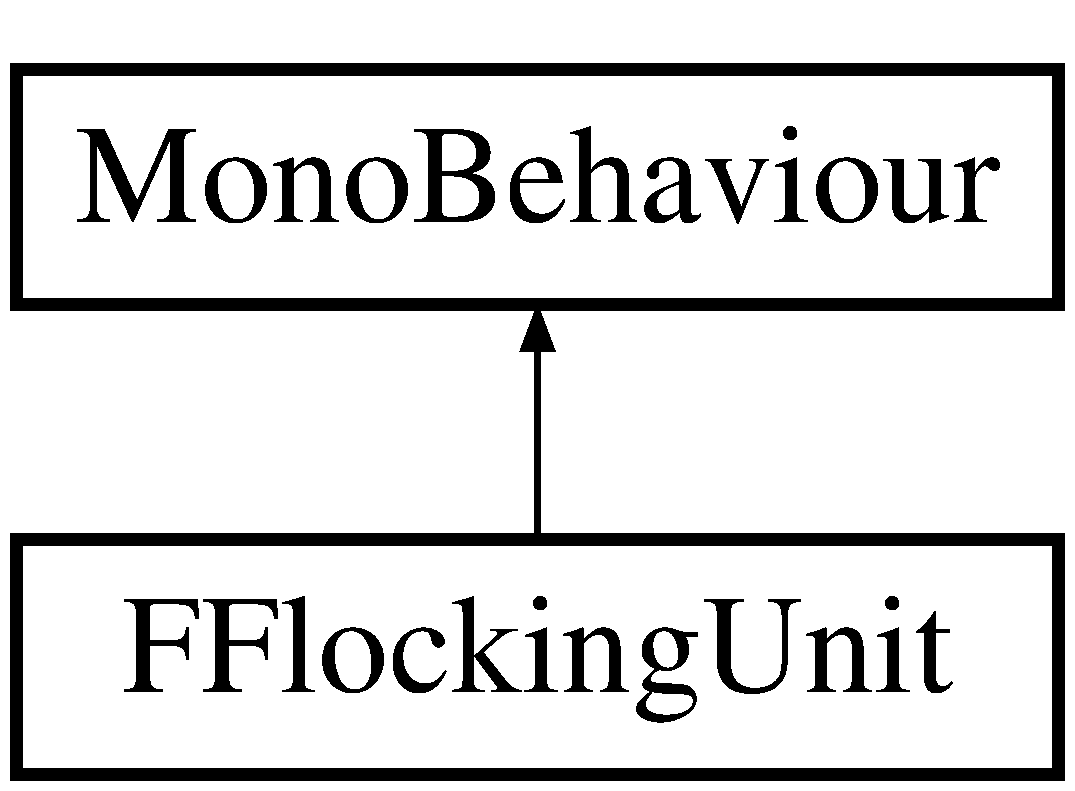
\includegraphics[height=2.000000cm]{class_f_flocking_unit}
\end{center}
\end{figure}
\subsection*{Public Attributes}
\begin{DoxyCompactItemize}
\item 
Game\+Object \hyperlink{class_f_flocking_unit_af63c7d39a0269bb66be7f75c7ee830be}{manager}
\begin{DoxyCompactList}\small\item\em Reference to the Manager Object which has the \hyperlink{class_f_unit_manager}{F\+Unit\+Manager} Script attached to it. \end{DoxyCompactList}\end{DoxyCompactItemize}
\subsection*{Protected Member Functions}
\begin{DoxyCompactItemize}
\item 
\mbox{\Hypertarget{class_f_flocking_unit_a2d94e65705a7536fc3c16b2013f9cc16}\label{class_f_flocking_unit_a2d94e65705a7536fc3c16b2013f9cc16}} 
void \hyperlink{class_f_flocking_unit_a2d94e65705a7536fc3c16b2013f9cc16}{Start} ()
\begin{DoxyCompactList}\small\item\em Called once from Unity. Do not call manually. Sets up variables needed later. \end{DoxyCompactList}\item 
void \hyperlink{class_f_flocking_unit_a86c5e9761219f7e36329f497406ef47b}{Update} ()
\begin{DoxyCompactList}\small\item\em Called periodically from Unity. Do not call manually. Makes the Boids look in the direction they are moving, calls the flock function and manages the Timer for the Goal-\/\+Velocity-\/\+Changer. \end{DoxyCompactList}\end{DoxyCompactItemize}


\subsection{Member Function Documentation}
\mbox{\Hypertarget{class_f_flocking_unit_a86c5e9761219f7e36329f497406ef47b}\label{class_f_flocking_unit_a86c5e9761219f7e36329f497406ef47b}} 
\index{F\+Flocking\+Unit@{F\+Flocking\+Unit}!Update@{Update}}
\index{Update@{Update}!F\+Flocking\+Unit@{F\+Flocking\+Unit}}
\subsubsection{\texorpdfstring{Update()}{Update()}}
{\footnotesize\ttfamily void F\+Flocking\+Unit.\+Update (\begin{DoxyParamCaption}{ }\end{DoxyParamCaption})\hspace{0.3cm}{\ttfamily [protected]}}



Called periodically from Unity. Do not call manually. Makes the Boids look in the direction they are moving, calls the flock function and manages the Timer for the Goal-\/\+Velocity-\/\+Changer. 

\begin{DoxySeeAlso}{See also}
flock() 
\end{DoxySeeAlso}


\subsection{Member Data Documentation}
\mbox{\Hypertarget{class_f_flocking_unit_af63c7d39a0269bb66be7f75c7ee830be}\label{class_f_flocking_unit_af63c7d39a0269bb66be7f75c7ee830be}} 
\index{F\+Flocking\+Unit@{F\+Flocking\+Unit}!manager@{manager}}
\index{manager@{manager}!F\+Flocking\+Unit@{F\+Flocking\+Unit}}
\subsubsection{\texorpdfstring{manager}{manager}}
{\footnotesize\ttfamily Game\+Object F\+Flocking\+Unit.\+manager}



Reference to the Manager Object which has the \hyperlink{class_f_unit_manager}{F\+Unit\+Manager} Script attached to it. 

Set this variable manually if \char`\"{}manual\+Start\char`\"{} is set in \hyperlink{class_f_unit_manager}{F\+Unit\+Manager}. 

The documentation for this class was generated from the following file\+:\begin{DoxyCompactItemize}
\item 
Assets/\+\_\+\+Scripts/F\+Flocking\+Unit.\+cs\end{DoxyCompactItemize}

\hypertarget{class_f_goal_random_movement}{}\section{F\+Goal\+Random\+Movement Class Reference}
\label{class_f_goal_random_movement}\index{F\+Goal\+Random\+Movement@{F\+Goal\+Random\+Movement}}
Inheritance diagram for F\+Goal\+Random\+Movement\+:\begin{figure}[H]
\begin{center}
\leavevmode
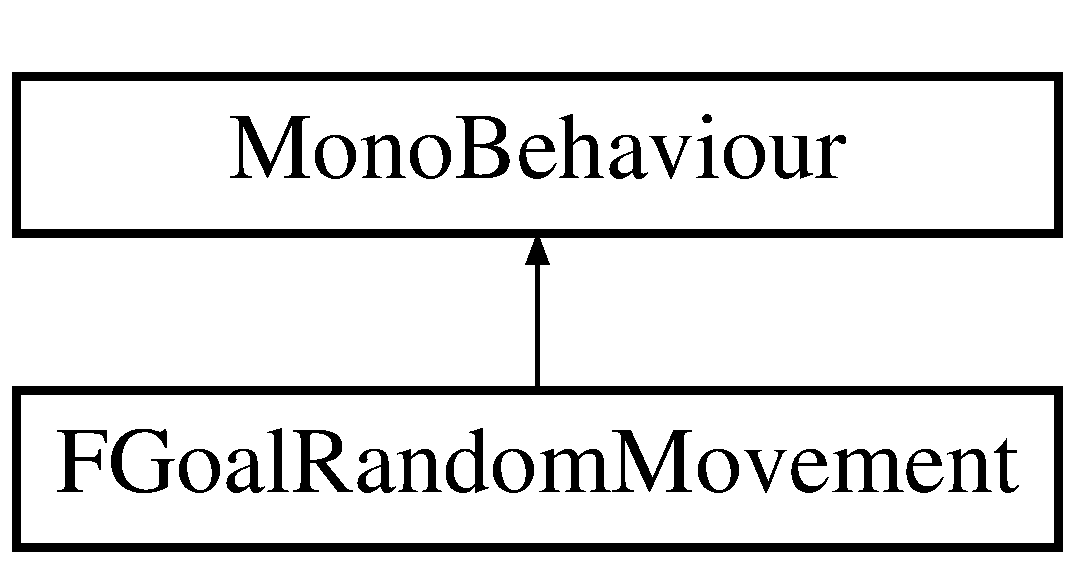
\includegraphics[height=2.000000cm]{class_f_goal_random_movement}
\end{center}
\end{figure}
\subsection*{Public Attributes}
\begin{DoxyCompactItemize}
\item 
\mbox{\Hypertarget{class_f_goal_random_movement_ab8e8d3b133e795e552e50bab68fa335b}\label{class_f_goal_random_movement_ab8e8d3b133e795e552e50bab68fa335b}} 
float {\bfseries speed} = 1.\+0f
\end{DoxyCompactItemize}


The documentation for this class was generated from the following file\+:\begin{DoxyCompactItemize}
\item 
Assets/\+\_\+\+Scripts/F\+Goal\+Random\+Movement.\+cs\end{DoxyCompactItemize}

\hypertarget{class_f_unit_manager}{}\section{F\+Unit\+Manager Class Reference}
\label{class_f_unit_manager}\index{F\+Unit\+Manager@{F\+Unit\+Manager}}
Inheritance diagram for F\+Unit\+Manager\+:\begin{figure}[H]
\begin{center}
\leavevmode
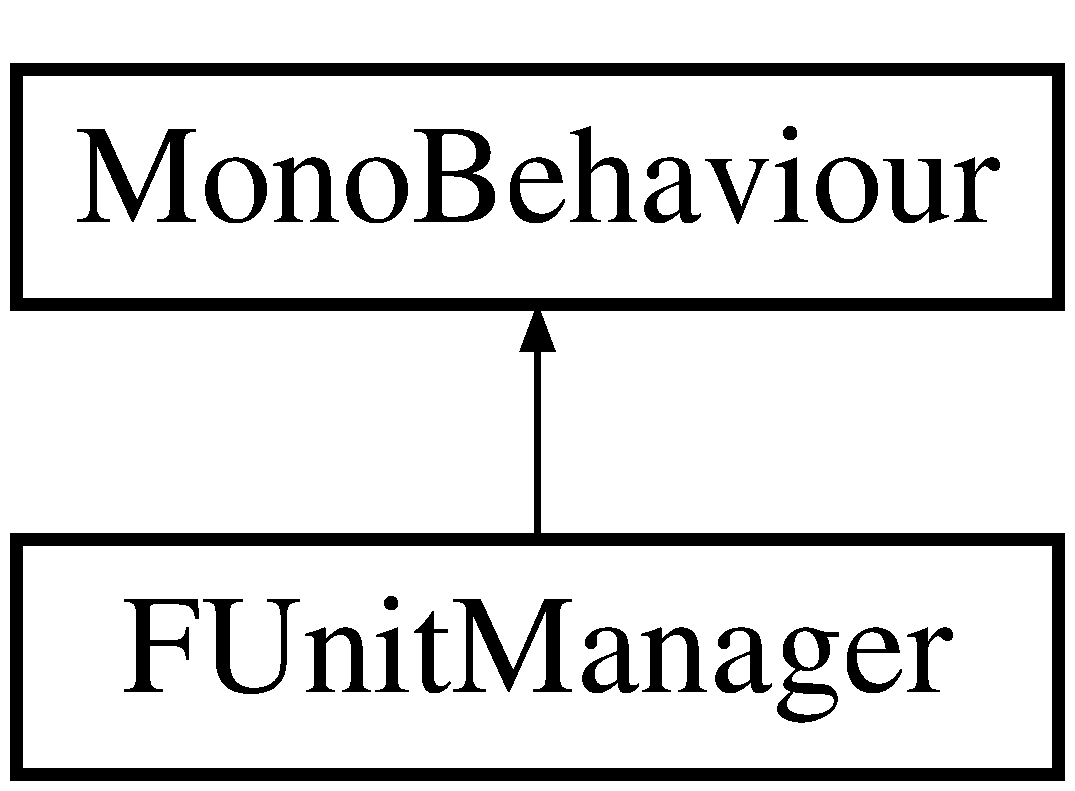
\includegraphics[height=2.000000cm]{class_f_unit_manager}
\end{center}
\end{figure}
\subsection*{Public Attributes}
\begin{DoxyCompactItemize}
\item 
\mbox{\Hypertarget{class_f_unit_manager_af516b428d69f61e7373d2e223ba2a9a9}\label{class_f_unit_manager_af516b428d69f61e7373d2e223ba2a9a9}} 
Game\+Object \mbox{[}$\,$\mbox{]} \hyperlink{class_f_unit_manager_af516b428d69f61e7373d2e223ba2a9a9}{units}
\begin{DoxyCompactList}\small\item\em Array holding the boids. \end{DoxyCompactList}\item 
\mbox{\Hypertarget{class_f_unit_manager_abdafb326f485fc9f68150a9a5d00ab6d}\label{class_f_unit_manager_abdafb326f485fc9f68150a9a5d00ab6d}} 
bool \hyperlink{class_f_unit_manager_abdafb326f485fc9f68150a9a5d00ab6d}{manual\+Start} = false
\begin{DoxyCompactList}\small\item\em Will not place any boids automatically in the scene. \end{DoxyCompactList}\item 
\mbox{\Hypertarget{class_f_unit_manager_a11b10c5e2eda939b9a408b878b0bf5d7}\label{class_f_unit_manager_a11b10c5e2eda939b9a408b878b0bf5d7}} 
Game\+Object \hyperlink{class_f_unit_manager_a11b10c5e2eda939b9a408b878b0bf5d7}{unit\+Prefab}
\begin{DoxyCompactList}\small\item\em Prefab Object from which the Boids will be created. \end{DoxyCompactList}\item 
\mbox{\Hypertarget{class_f_unit_manager_a042d6edcb06e9b9c79c56e4cc722d385}\label{class_f_unit_manager_a042d6edcb06e9b9c79c56e4cc722d385}} 
int \hyperlink{class_f_unit_manager_a042d6edcb06e9b9c79c56e4cc722d385}{num\+Units} = 100
\begin{DoxyCompactList}\small\item\em Number of Boids that will be created. \end{DoxyCompactList}\item 
\mbox{\Hypertarget{class_f_unit_manager_a96ce82693289e9fded138cf1f59c4c40}\label{class_f_unit_manager_a96ce82693289e9fded138cf1f59c4c40}} 
Vector3 \hyperlink{class_f_unit_manager_a96ce82693289e9fded138cf1f59c4c40}{spawn\+Range} = new Vector3(10.\+0f, 5f, 10.\+0f)
\begin{DoxyCompactList}\small\item\em The Spawnrange in which the Boids will be instantiated. \end{DoxyCompactList}\item 
\mbox{\Hypertarget{class_f_unit_manager_a43c285fed4df2253698b2f9e472e3add}\label{class_f_unit_manager_a43c285fed4df2253698b2f9e472e3add}} 
Game\+Object \hyperlink{class_f_unit_manager_a43c285fed4df2253698b2f9e472e3add}{goal}
\begin{DoxyCompactList}\small\item\em A Goal the Boids will follow, if seek\+Goal is set to true. \end{DoxyCompactList}\item 
\mbox{\Hypertarget{class_f_unit_manager_a79d01dac80c57300f39750b6f6d920eb}\label{class_f_unit_manager_a79d01dac80c57300f39750b6f6d920eb}} 
bool \hyperlink{class_f_unit_manager_a79d01dac80c57300f39750b6f6d920eb}{seek\+Goal} = true
\begin{DoxyCompactList}\small\item\em If set to true, the Boids will follow the \char`\"{}goal\char`\"{} Game\+Object. \end{DoxyCompactList}\item 
\mbox{\Hypertarget{class_f_unit_manager_ae2bb63f32195acc71f88cdf7c656fd44}\label{class_f_unit_manager_ae2bb63f32195acc71f88cdf7c656fd44}} 
bool \hyperlink{class_f_unit_manager_ae2bb63f32195acc71f88cdf7c656fd44}{obedient} = true
\begin{DoxyCompactList}\small\item\em Will apply random forces to boids from time to time, if set to true. \end{DoxyCompactList}\item 
\mbox{\Hypertarget{class_f_unit_manager_a120a66886a707186f5d8de29d4d4fcba}\label{class_f_unit_manager_a120a66886a707186f5d8de29d4d4fcba}} 
float \hyperlink{class_f_unit_manager_a120a66886a707186f5d8de29d4d4fcba}{max\+Force} = 4.\+0f
\begin{DoxyCompactList}\small\item\em The maximum Force that will be applied to the Boids. \end{DoxyCompactList}\item 
\mbox{\Hypertarget{class_f_unit_manager_acf8af35dd5ba76af298dd14a941116cd}\label{class_f_unit_manager_acf8af35dd5ba76af298dd14a941116cd}} 
float \hyperlink{class_f_unit_manager_acf8af35dd5ba76af298dd14a941116cd}{maxvelocity} = 2.\+0f
\begin{DoxyCompactList}\small\item\em The maximum Velocity the Boids can reach. \end{DoxyCompactList}\item 
\mbox{\Hypertarget{class_f_unit_manager_a6fffed9f8949e5908b5ff789779b8abb}\label{class_f_unit_manager_a6fffed9f8949e5908b5ff789779b8abb}} 
float \hyperlink{class_f_unit_manager_a6fffed9f8949e5908b5ff789779b8abb}{alignment\+Strength} = 0.\+5f
\begin{DoxyCompactList}\small\item\em Sets how much the Boids will align to each other. \end{DoxyCompactList}\item 
\mbox{\Hypertarget{class_f_unit_manager_a58ef6cb569af68ab076ea7ba13920620}\label{class_f_unit_manager_a58ef6cb569af68ab076ea7ba13920620}} 
float \hyperlink{class_f_unit_manager_a58ef6cb569af68ab076ea7ba13920620}{alignment\+Distance} = 6
\begin{DoxyCompactList}\small\item\em The maximum distance that Boids can be away from each other to make alignmet work. \end{DoxyCompactList}\item 
\mbox{\Hypertarget{class_f_unit_manager_ab81d3274a3cd1fbd52bea96df052dac4}\label{class_f_unit_manager_ab81d3274a3cd1fbd52bea96df052dac4}} 
float \hyperlink{class_f_unit_manager_ab81d3274a3cd1fbd52bea96df052dac4}{cohesion\+Strength} = 0.\+5f
\begin{DoxyCompactList}\small\item\em Sets how much the Boids will stick to each other. \end{DoxyCompactList}\item 
\mbox{\Hypertarget{class_f_unit_manager_a4288c71deee22c3f89aa418ea31294bb}\label{class_f_unit_manager_a4288c71deee22c3f89aa418ea31294bb}} 
float \hyperlink{class_f_unit_manager_a4288c71deee22c3f89aa418ea31294bb}{cohesion\+Distance} = 6
\begin{DoxyCompactList}\small\item\em The maximum distance that Boids can be away from each other to make cohesion work. \end{DoxyCompactList}\item 
\mbox{\Hypertarget{class_f_unit_manager_a592278d1412ee25871d11b26cfca66e6}\label{class_f_unit_manager_a592278d1412ee25871d11b26cfca66e6}} 
float \hyperlink{class_f_unit_manager_a592278d1412ee25871d11b26cfca66e6}{separation\+Strength} = 0.\+5f
\begin{DoxyCompactList}\small\item\em Sets how much the Boids will try to move away from each other. \end{DoxyCompactList}\item 
\mbox{\Hypertarget{class_f_unit_manager_a99ced2e66851fd9dc1356935710cb315}\label{class_f_unit_manager_a99ced2e66851fd9dc1356935710cb315}} 
float \hyperlink{class_f_unit_manager_a99ced2e66851fd9dc1356935710cb315}{separation\+Distance} = 5
\begin{DoxyCompactList}\small\item\em The maximum distance that Boids can be away from each other to make separation work. \end{DoxyCompactList}\item 
\mbox{\Hypertarget{class_f_unit_manager_a4e7f24e9faeda6f66ab7f5a6d193cff6}\label{class_f_unit_manager_a4e7f24e9faeda6f66ab7f5a6d193cff6}} 
float \hyperlink{class_f_unit_manager_a4e7f24e9faeda6f66ab7f5a6d193cff6}{randomizer\+Strength} = 0.\+2f
\begin{DoxyCompactList}\small\item\em Sets how much randomized Force should be applied to the Boids. \end{DoxyCompactList}\item 
\mbox{\Hypertarget{class_f_unit_manager_ad341d31117c315aa6c66bfd8fb6e848b}\label{class_f_unit_manager_ad341d31117c315aa6c66bfd8fb6e848b}} 
float \hyperlink{class_f_unit_manager_ad341d31117c315aa6c66bfd8fb6e848b}{viewing\+Angle} = 170.\+0f
\begin{DoxyCompactList}\small\item\em The angle in which a Boid can \char`\"{}see\char`\"{} others. Cohesion, Alignment, Separation will only be applied if Boids are within the viewing Angle. \end{DoxyCompactList}\end{DoxyCompactItemize}


The documentation for this class was generated from the following file\+:\begin{DoxyCompactItemize}
\item 
Assets/\+\_\+\+Scripts/F\+Unit\+Manager.\+cs\end{DoxyCompactItemize}

\hypertarget{class_unit_manager}{}\section{Unit\+Manager Class Reference}
\label{class_unit_manager}\index{Unit\+Manager@{Unit\+Manager}}
Inheritance diagram for Unit\+Manager\+:\begin{figure}[H]
\begin{center}
\leavevmode
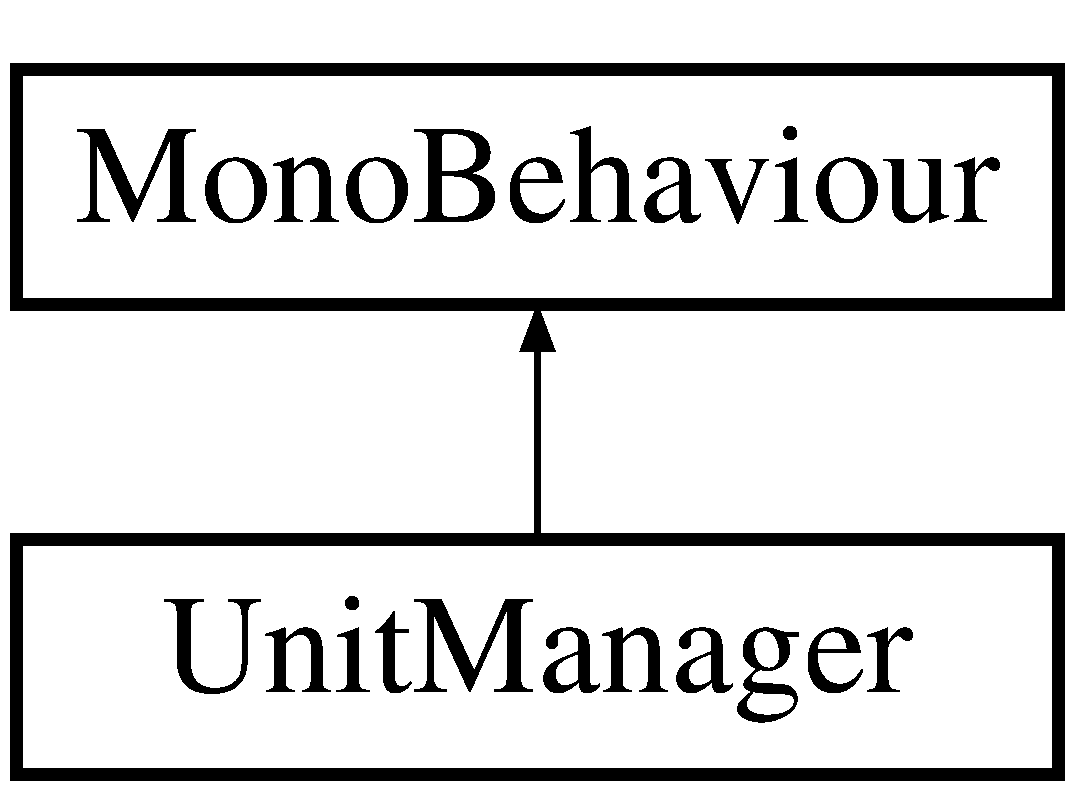
\includegraphics[height=2.000000cm]{class_unit_manager}
\end{center}
\end{figure}
\subsection*{Public Attributes}
\begin{DoxyCompactItemize}
\item 
\mbox{\Hypertarget{class_unit_manager_ae3b00f134786d65f4d2596b5dea72b27}\label{class_unit_manager_ae3b00f134786d65f4d2596b5dea72b27}} 
Game\+Object \mbox{[}$\,$\mbox{]} {\bfseries units}
\item 
\mbox{\Hypertarget{class_unit_manager_ae9ce302388b9ca7614bda98ae6771a32}\label{class_unit_manager_ae9ce302388b9ca7614bda98ae6771a32}} 
Game\+Object {\bfseries unit\+Prefab}
\item 
\mbox{\Hypertarget{class_unit_manager_a903b6a94b80a74492b0fa09b87f85cbf}\label{class_unit_manager_a903b6a94b80a74492b0fa09b87f85cbf}} 
int {\bfseries num\+Units} = 100
\item 
\mbox{\Hypertarget{class_unit_manager_a9a4c1f152ee3731c67475a4dc0bf88fc}\label{class_unit_manager_a9a4c1f152ee3731c67475a4dc0bf88fc}} 
Vector3 {\bfseries range} = new Vector3 (10.\+0f, 5f, 10.\+0f)
\item 
\mbox{\Hypertarget{class_unit_manager_af71ea57608f99a8011ef4861ce35bd5f}\label{class_unit_manager_af71ea57608f99a8011ef4861ce35bd5f}} 
bool {\bfseries seek\+Goal} = true
\item 
\mbox{\Hypertarget{class_unit_manager_a47231b058515f2e03f40adfa7be1d8f2}\label{class_unit_manager_a47231b058515f2e03f40adfa7be1d8f2}} 
bool {\bfseries obedient} = true
\item 
\mbox{\Hypertarget{class_unit_manager_a3e6616b3089da5dfc42d472025a4cc88}\label{class_unit_manager_a3e6616b3089da5dfc42d472025a4cc88}} 
bool {\bfseries willful} = false
\item 
\mbox{\Hypertarget{class_unit_manager_aa888e707617707fc3d4754bf8bfb4732}\label{class_unit_manager_aa888e707617707fc3d4754bf8bfb4732}} 
int {\bfseries neighbour\+Distance} = 50
\item 
\mbox{\Hypertarget{class_unit_manager_abfc2eb72073d21b463119c3baf317e50}\label{class_unit_manager_abfc2eb72073d21b463119c3baf317e50}} 
float {\bfseries max\+Force} = 0.\+5f
\item 
\mbox{\Hypertarget{class_unit_manager_af2bf30735657c5644286491665feaabb}\label{class_unit_manager_af2bf30735657c5644286491665feaabb}} 
float {\bfseries maxvelocity} = 2.\+0f
\item 
\mbox{\Hypertarget{class_unit_manager_a12c55a004abe173415b84e29a28a9997}\label{class_unit_manager_a12c55a004abe173415b84e29a28a9997}} 
float {\bfseries alignment} = 0.\+5f
\end{DoxyCompactItemize}


The documentation for this class was generated from the following file\+:\begin{DoxyCompactItemize}
\item 
Assets/\+\_\+\+Scripts/Unit\+Manager.\+cs\end{DoxyCompactItemize}

%--- End generated contents ---

% Index
\backmatter
\newpage
\phantomsection
\clearemptydoublepage
\addcontentsline{toc}{chapter}{Index}
\printindex

\end{document}
